\documentclass[aspectratio=169,10pt]{beamer}

\usepackage[utf8]{inputenc}
\usepackage[T1]{fontenc}
\usepackage[brazilian]{babel}
\usepackage{lmodern}
\usepackage{graphicx}
\usepackage{booktabs}
\usepackage{array}
\usepackage{colortbl}
\usepackage{tikz}
\usepackage{pgfplots}
\usepackage{pgfplotstable}
\usepackage{url}
\usetikzlibrary{arrows.meta,calc,positioning,shapes.geometric,fit}
\pgfplotsset{compat=1.18}

\definecolor{ufpiBlue}{HTML}{1E4F8F}
\definecolor{ufpiGold}{HTML}{F4C430}
\definecolor{ink}{HTML}{172033}
\definecolor{muted}{HTML}{5E6A7D}
\definecolor{lineGray}{HTML}{D8DEE8}
\definecolor{softBlue}{HTML}{F3F6FA}
\definecolor{softGold}{HTML}{FBF6E6}
\definecolor{softGreen}{HTML}{F2F6F3}
\definecolor{softRed}{HTML}{F7F1F1}
\definecolor{tpGreen}{HTML}{2F7D50}
\definecolor{fpOrange}{HTML}{B66A2C}
\definecolor{fnRed}{HTML}{A83A34}

\graphicspath{{media/}{../sbc-final/figuras/}{../../results/article_materials/figuras/}}
\urlstyle{same}

\setbeamertemplate{navigation symbols}{}
\setbeamertemplate{caption}[numbered]
\setbeamercolor{normal text}{fg=ink,bg=white}
\setbeamercolor{frametitle}{fg=ink,bg=white}
\setbeamerfont{frametitle}{series=\bfseries,size=\Large}
\setbeamerfont{title}{series=\bfseries,size=\Large}
\setbeamerfont{subtitle}{size=\normalsize}
\setbeamercolor{itemize item}{fg=ufpiBlue}
\setbeamercolor{itemize subitem}{fg=ufpiBlue}
\setbeamertemplate{itemize item}{\raise0.2ex\hbox{\small$\blacktriangleright$}}
\setbeamertemplate{itemize subitem}{\raise0.2ex\hbox{\scriptsize$\bullet$}}

\newif\ifbackup
\backupfalse
\newcommand{\mainSlideTotal}{19}
\setbeamertemplate{footline}{%
  \leavevmode%
  \hbox{%
    \begin{beamercolorbox}[wd=.72\paperwidth,ht=2.8ex,dp=1.1ex,leftskip=1.2em]{author in head/foot}%
      \scriptsize\color{muted}Detecção e Contagem de Células Cervicais
    \end{beamercolorbox}%
    \begin{beamercolorbox}[wd=.28\paperwidth,ht=2.8ex,dp=1.1ex,rightskip=1.2em plus1fil]{date in head/foot}%
      \hfill\scriptsize\color{muted}\ifbackup Backup \insertframenumber\else \insertframenumber/\mainSlideTotal\fi
    \end{beamercolorbox}%
  }%
}

\newcommand{\accentbar}{%
  \begin{tikzpicture}[remember picture,overlay]
    \fill[ufpiBlue] (current page.north west) rectangle ([yshift=-2.2pt]current page.north east);
    \fill[ufpiGold] (current page.north west) rectangle ([xshift=.24\paperwidth,yshift=-2.2pt]current page.north west);
  \end{tikzpicture}%
}

\newcommand{\tightframe}[1]{\begin{frame}[t]{#1}\accentbar}
\newcommand{\source}[1]{\vfill{\scriptsize\color{muted}#1}}

\newcommand{\metriccard}[4]{%
  \begin{tikzpicture}
    \node[
      draw=#1!50,
      fill=white,
      rounded corners=5pt,
      minimum width=2.75cm,
      minimum height=1.58cm,
      align=center,
      inner sep=5pt
    ] {
      {\scriptsize\color{muted}#2}\\[-1pt]
      {\Large\bfseries\color{ink}#3}\\[-1pt]
      {\scriptsize\color{muted}#4}
    };
  \end{tikzpicture}%
}

\newcommand{\phasebox}[4]{%
  \node[
    draw=#1!55,
    fill=white,
    rounded corners=5pt,
    minimum width=2.25cm,
    minimum height=1.1cm,
    align=center,
    font=\small,
    inner sep=4pt
  ] (#2) {#3\\[-2pt]{\scriptsize\color{muted}#4}};
}

\newcommand{\cellcluster}[1]{%
  \begin{tikzpicture}[scale=#1]
    \foreach \x/\y/\r/\c in {
      0/0/.32/softBlue, .42/.18/.25/softGold, -.38/.18/.27/softGreen,
      .15/-.35/.22/softRed, -.18/.43/.22/softBlue, .72/-.23/.2/softGreen,
      -.72/-.23/.21/softGold} {
      \fill[\c,draw=ufpiBlue!30,line width=.3pt] (\x,\y) circle (\r);
      \fill[ufpiBlue!75] (\x,\y) circle (.045);
    }
  \end{tikzpicture}%
}

\newcommand{\rqcard}[3]{%
  \begin{tikzpicture}
    \node[
      draw=lineGray,
      fill=white,
      rounded corners=5pt,
      minimum width=3.75cm,
      minimum height=2.15cm,
      align=left,
      text width=3.35cm,
      inner sep=8pt
    ] {
      {\large\bfseries\color{ufpiBlue}#1}\\[4pt]
      {\bfseries #2}\\[2pt]
      {\scriptsize\color{muted}#3}
    };
  \end{tikzpicture}%
}

\title{Detecção e Contagem de Células Cervicais a partir de Anotações Pontuais}
\author{Jean Carlos Rodrigues Sousa}
\institute{Universidade Federal do Piauí -- Campus Senador Helvídio Nunes de Barros}
\date{Trabalho Final}

\begin{document}

% 1
\begin{frame}[plain]
\begin{tikzpicture}[remember picture,overlay]
  \fill[white] (current page.south west) rectangle (current page.north east);
  \fill[ufpiBlue] (current page.north west) rectangle ([yshift=-4pt]current page.north east);
  \fill[ufpiGold] (current page.north west) rectangle ([xshift=.30\paperwidth,yshift=-4pt]current page.north west);
  \node[anchor=north east,inner sep=0pt] at ([xshift=-.75cm,yshift=-.62cm]current page.north east)
    {
\includegraphics[height=1.75cm]{image.png}};
  \node[anchor=west,align=left,text width=10.6cm] at ([xshift=.85cm,yshift=.85cm]current page.west) {
    {\Large\bfseries\color{ink}Detecção e Contagem de Células Cervicais}\\[2pt]
    {\Large\bfseries\color{ink}a partir de Anotações Pontuais}\\[12pt]
    {\normalsize\color{muted}Disciplina: Sistemas Inteligentes}\\[22pt]
    {\bfseries Jean Carlos Rodrigues Sousa}\\[5pt]
    {\small Coorientador: João Antônio Leal de Miranda}\\
    {\small Orientador: Romuere Rodrigues Veloso e Silva}\\[12pt]
    {\small Universidade Federal do Piauí (UFPI)}\\
    {\small Campus Senador Helvídio Nunes de Barros (CSHNB)}
  };
  \node[anchor=south east,inner sep=0pt,draw=lineGray,line width=.4pt] at ([xshift=-.65cm,yshift=.45cm]current page.south east)
    {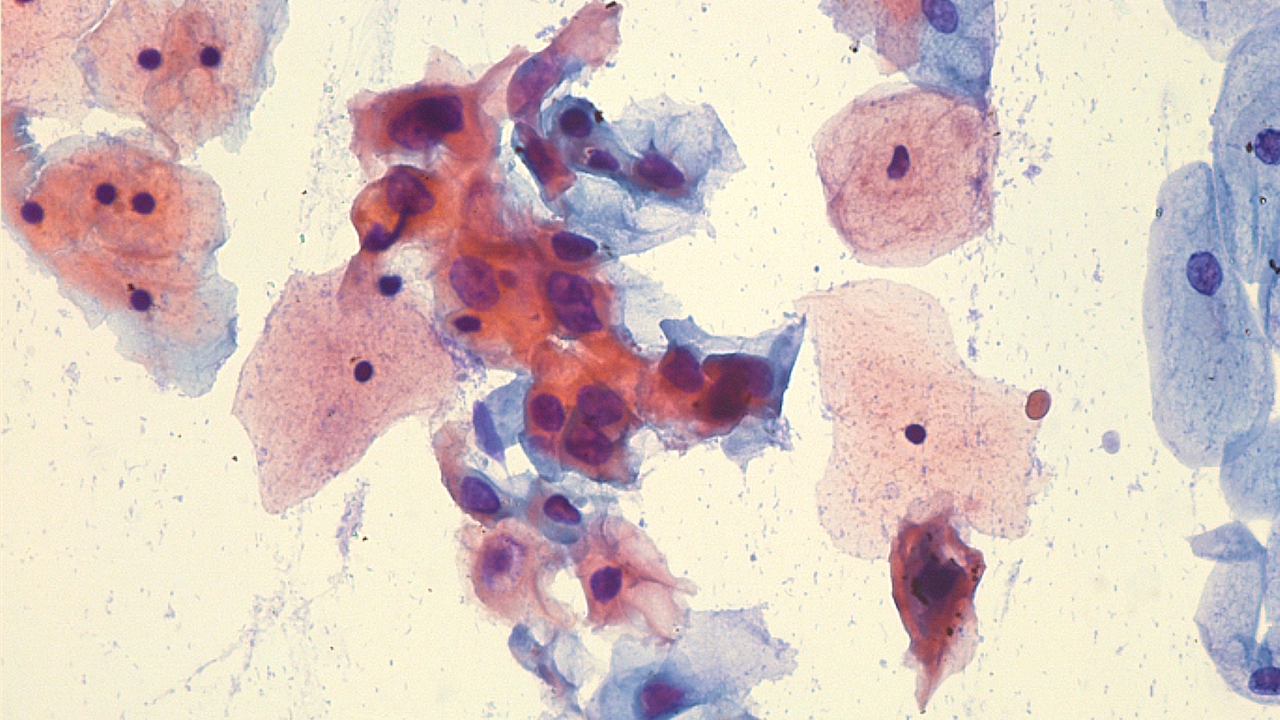
\includegraphics[width=4.1cm]{cric_context.png}};
\end{tikzpicture}
\end{frame}

% 2
\tightframe{Motivação}
\begin{columns}[T,totalwidth=\textwidth]
\column{.45\textwidth}
\metriccard{fnRed}{Novos casos em 2020}{604 mil}{mundo}
\hspace{.25cm}
\metriccard{fnRed}{Óbitos em 2020}{342 mil}{mundo}

\vspace{.45cm}
\begin{itemize}
  \item Citologia cervical apoia o rastreamento.
  \item A automação pode auxiliar triagem, revisão e priorização.
  \item Para isso, é preciso localizar e contar células em campos complexos.
\end{itemize}
\source{Base epidemiológica: Singh et al. (2023).}

\column{.55\textwidth}
\centering
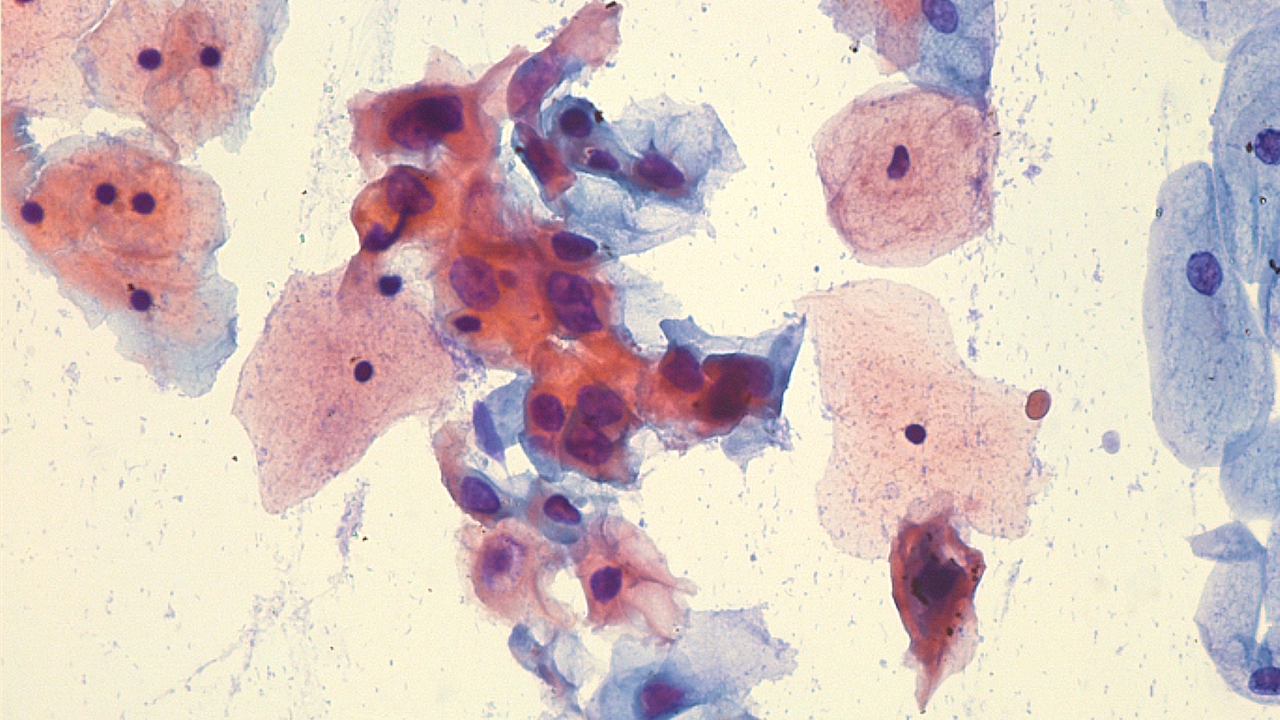
\includegraphics[width=\linewidth]{cric_context.png}
\vspace{.12cm}

{\scriptsize\color{muted}Exemplo real da CRIC Cervix: campo citológico com variação morfológica e densidade celular.}
\end{columns}
\end{frame}

% 3
\tightframe{Do exame à contagem}
\begin{columns}[T,totalwidth=\textwidth]
\column{.44\textwidth}
\vspace{.1cm}
{\Large\bfseries O problema não começa no modelo.}

\vspace{.32cm}
{\color{muted}O trabalho parte de uma anotação simples, o ponto nuclear, e constrói um caminho reprodutível até detecção e contagem por imagem.}

\vspace{.45cm}
\begin{itemize}
  \item Imagem de citologia: muitas células por campo.
  \item Anotação disponível: coordenada do núcleo.
  \item Saída desejada: localização e contagem por imagem.
\end{itemize}

\column{.56\textwidth}
\centering
\begin{tikzpicture}[>=Latex]
  \node[draw=lineGray,fill=white,rounded corners=5pt,minimum width=2.55cm,minimum height=1.12cm,align=center] (img) at (0,0)
    {\bfseries Imagem\\[-1pt]{\scriptsize\color{muted}citologia}};
  \node[draw=lineGray,fill=white,rounded corners=5pt,minimum width=2.55cm,minimum height=1.12cm,align=center] (ann) at (3.15,0)
    {\bfseries Ponto\\[-1pt]{\scriptsize\color{muted}núcleo anotado}};
  \node[draw=lineGray,fill=white,rounded corners=5pt,minimum width=2.55cm,minimum height=1.12cm,align=center] (target) at (0,-1.7)
    {\bfseries Treino\\[-1pt]{\scriptsize\color{muted}a partir do ponto}};
  \node[draw=lineGray,fill=white,rounded corners=5pt,minimum width=2.55cm,minimum height=1.12cm,align=center] (out) at (3.15,-1.7)
    {\bfseries Saída\\[-1pt]{\scriptsize\color{muted}detecção + contagem}};
  \draw[->,thick,ufpiBlue!80] (img) -- (ann);
  \draw[->,thick,ufpiBlue!80] (ann.south) to[out=-90,in=90] (target.north);
  \draw[->,thick,ufpiBlue!80] (target) -- (out);
  \node[anchor=north,align=center,text width=6.55cm,font=\small\color{muted}] at (1.55,-2.55)
    {A contribuição é integrar anotação pontual, detector e leitura operacional em um protocolo auditável.};
\end{tikzpicture}

\vspace{.35cm}
\begin{tikzpicture}
  \node[draw=ufpiBlue!45,fill=white,rounded corners=6pt,text width=6.7cm,align=center,inner sep=8pt]
    {\bfseries Detecção e contagem de células cervicais\\a partir de anotações pontuais.};
\end{tikzpicture}
\end{columns}
\end{frame}

% 4
\tightframe{Da anotação pontual à detecção}
\centering
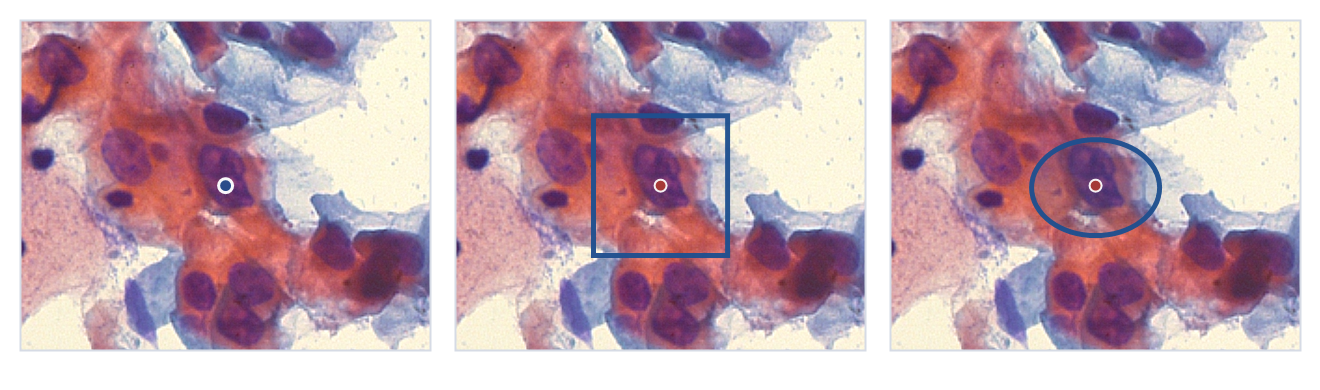
\includegraphics[width=.94\linewidth]{cric_annotation_comparison.png}

\vspace{.12cm}
\begin{tikzpicture}
  \node[text width=3.55cm,align=center,font=\bfseries\color{ufpiBlue}] at (0,0) {Ponto};
  \node[text width=3.55cm,align=center,font=\bfseries\color{ufpiBlue}] at (4.25,0) {Ponto adaptado};
  \node[text width=3.55cm,align=center,font=\bfseries\color{ufpiBlue}] at (8.5,0) {Máscara};
  \node[text width=3.55cm,align=center,font=\scriptsize\color{muted}] at (0,-.55) {barato, mas sem extensão};
  \node[text width=3.55cm,align=center,font=\scriptsize\color{muted}] at (4.25,-.55) {ponte entre ponto e detector};
  \node[text width=3.55cm,align=center,font=\scriptsize\color{muted}] at (8.5,-.55) {detalhada, mas ausente na CRIC};
\end{tikzpicture}
\vspace{.15cm}

{\large\bfseries O desafio é transformar pontos em localização e contagem avaliáveis.}
\end{frame}

% 5
\tightframe{Base CRIC Cervix}
\begin{columns}[T,totalwidth=\textwidth]
\column{.45\textwidth}
\metriccard{ufpiBlue}{Imagens}{400}{Papanicolau}
\hspace{.25cm}
\metriccard{ufpiBlue}{Células}{11.534}{coordenadas}

\vspace{.45cm}
\begin{itemize}
  \item Coordenadas nucleares como supervisão espacial.
  \item Categorias Bethesda preservadas nos metadados.
  \item Treinamento como classe única: \textit{cell}.
\end{itemize}

\column{.55\textwidth}
\centering
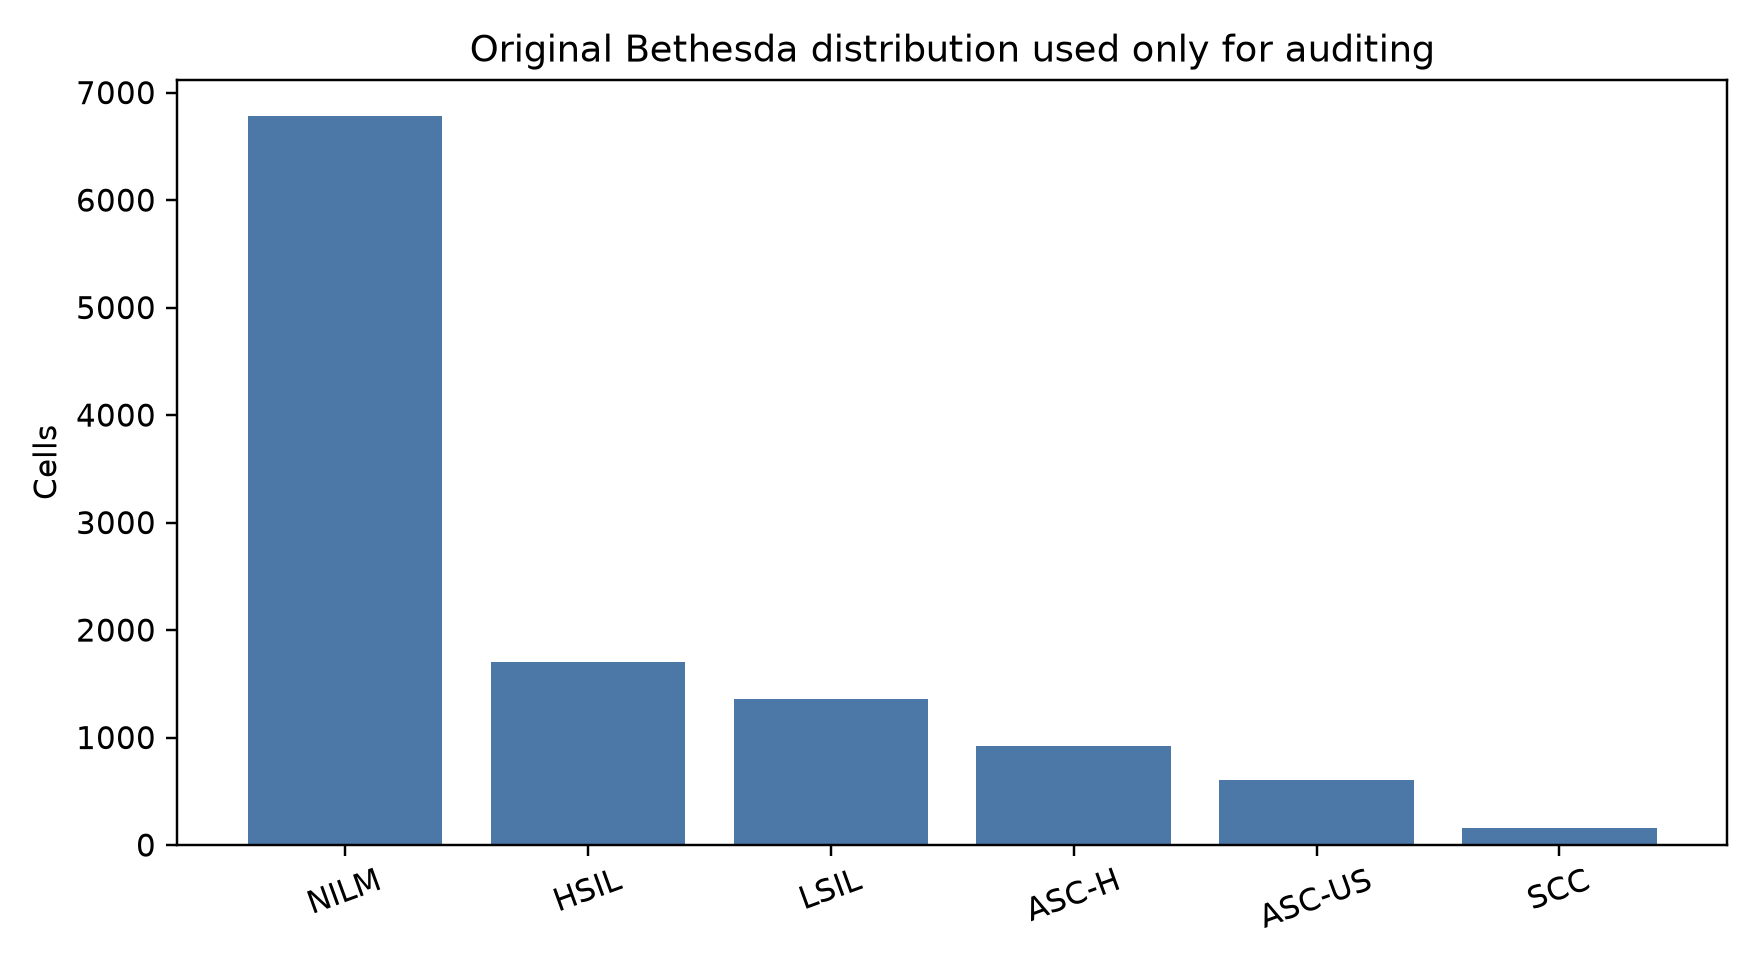
\includegraphics[width=.86\linewidth]{fig_composicao_bethesda_original.png}
\vspace{.1cm}

{\scriptsize\color{muted}Composição usada para auditoria; não como alvo de classificação.}
\end{columns}
\end{frame}

% 6
\tightframe{Lacuna}
\begin{columns}[T,totalwidth=\textwidth]
\column{.48\textwidth}
{\Large\bfseries A base entrega pontos; o sistema precisa entregar detecções.}

\vspace{.22cm}
\begin{tikzpicture}[
  box/.style={draw=ufpiBlue!45,fill=white,rounded corners=7pt,
    text width=4.95cm,minimum height=1.02cm,align=center,inner sep=6pt},
  arr/.style={-{Latex[length=2mm]},ufpiBlue!70,thick}
]
  \node[box] (in) at (0,0) {\bfseries Entrada\\[-1pt]{\small\color{muted}pontos nucleares}};
  \node[box,draw=ufpiGold!75] (mid) at (0,-1.38) {\bfseries Etapa crítica\\[-1pt]{\small\color{muted}treinar o detector}};
  \node[box,draw=tpGreen!60] (out) at (0,-2.76) {\bfseries Saída\\[-1pt]{\small\color{muted}localização + contagem}};
  \draw[arr] (in) -- (mid);
  \draw[arr] (mid) -- (out);
\end{tikzpicture}

\column{.52\textwidth}
{\Large\bfseries O que precisava ser medido?}

\vspace{.18cm}
\begin{tikzpicture}
  \node[draw=ufpiBlue!45,fill=softBlue,rounded corners=8pt,
    text width=6.0cm,align=left,inner sep=8pt] {
    {\bfseries Pergunta do trabalho}\\[4pt]
    {\large Como sair de pontos anotados para um detector que localiza e conta células de forma confiável?}
  };
\end{tikzpicture}

\vspace{.28cm}
\begin{itemize}
  \item Se os pontos bastam para treinar um detector útil.
  \item Como o treino afeta acertos, FP, FN e contagem.
  \item Se a escolha se mantém em teste retido.
\end{itemize}
\end{columns}
\end{frame}

% 7
\tightframe{Perguntas de pesquisa}
\centering
\rqcard{RQ1}{Uso dos pontos}{Pontos bastam para localizar e contar?}
\hspace{.25cm}
\rqcard{RQ2}{Escala YOLO11}{Modelo maior melhora o compromisso operacional?}
\hspace{.25cm}
\rqcard{RQ3}{Teste retido}{A escolha mantém desempenho fora da validação?}

\vspace{.55cm}
\begin{tikzpicture}[>=Latex]
  \draw[thick,ufpiBlue!65,->] (0,0) -- (10.5,0);
  \foreach \x/\lab in {0.5/RQ1,4.9/RQ2,9.2/RQ3} {
    \fill[ufpiGold] (\x,0) circle (.08);
    \node[above=.13cm,font=\bfseries,text=ufpiBlue] at (\x,0) {\lab};
  }
  \node[below=.12cm,font=\scriptsize\color{muted}] at (.5,0) {pontos};
  \node[below=.12cm,font=\scriptsize\color{muted}] at (4.9,0) {capacidade};
  \node[below=.12cm,font=\scriptsize\color{muted}] at (9.2,0) {generalização};
\end{tikzpicture}
\end{frame}

% 8
\tightframe{Pipeline experimental}
\centering
\begin{tikzpicture}[
  >=Latex,
  box/.style={draw=ufpiBlue!45,fill=white,rounded corners=7pt,
    minimum height=1.02cm,align=center,font=\small,inner sep=5pt},
  note/.style={draw=lineGray,fill=white,rounded corners=7pt,
    align=center,font=\small,inner sep=7pt},
  arr/.style={->,thick,ufpiBlue!70}
]
  \node[box,minimum width=1.6cm] (cric) at (0,1.25) {CRIC\\[-2pt]{\scriptsize\color{muted}400 imagens}};
  \node[box,minimum width=1.7cm,draw=ufpiGold!70] (split) at (2.15,1.25) {Partição\\[-2pt]{\scriptsize\color{muted}por imagem}};

  \node[box,minimum width=1.55cm,draw=tpGreen!65] (trainset) at (4.25,1.95) {Treino\\[-2pt]{\scriptsize\color{muted}320}};
  \node[box,minimum width=1.55cm,draw=fpOrange!65] (valset) at (4.25,.55) {Validação\\[-2pt]{\scriptsize\color{muted}40}};
  \node[box,minimum width=1.55cm,draw=fnRed!65] (testset) at (4.25,-1.05) {Teste\\[-2pt]{\scriptsize\color{muted}40}};

  \node[box,minimum width=2.25cm,draw=tpGreen!65] (train) at (6.75,1.95) {Treinar YOLO11\\[-2pt]{\scriptsize\color{muted}pontos + região}};
  \node[box,minimum width=2.55cm,draw=fpOrange!65] (choose) at (8.95,.55) {Escolher configuração\\[-2pt]{\scriptsize\color{muted}região, escala, limiar}};
  \node[box,minimum width=2.45cm,draw=fnRed!65] (final) at (8.95,-1.05) {Avaliação final\\[-2pt]{\scriptsize\color{muted}localização + contagem}};

  \draw[arr] (cric) -- (split);
  \draw[arr] (split) -- (trainset);
  \draw[arr] (split) -- (valset);
  \draw[arr] (split) -- (testset);
  \draw[arr] (trainset) -- (train);
  \draw[arr] (train) -- (choose);
  \draw[arr] (valset) -- (choose);
  \draw[arr] (choose) -- (final);
  \draw[arr] (testset) -- (final);

  \node[note,text width=8.2cm] at (5.65,-2.35)
    {\bfseries Sem vazamento de teste: \normalfont o teste retido não decide parâmetros; ele só mede o desempenho final da configuração escolhida na validação.};
\end{tikzpicture}
\end{frame}

% 9
\tightframe{Como treinar com pontos}
\begin{columns}[T,totalwidth=\textwidth]
\column{.5\textwidth}
\centering
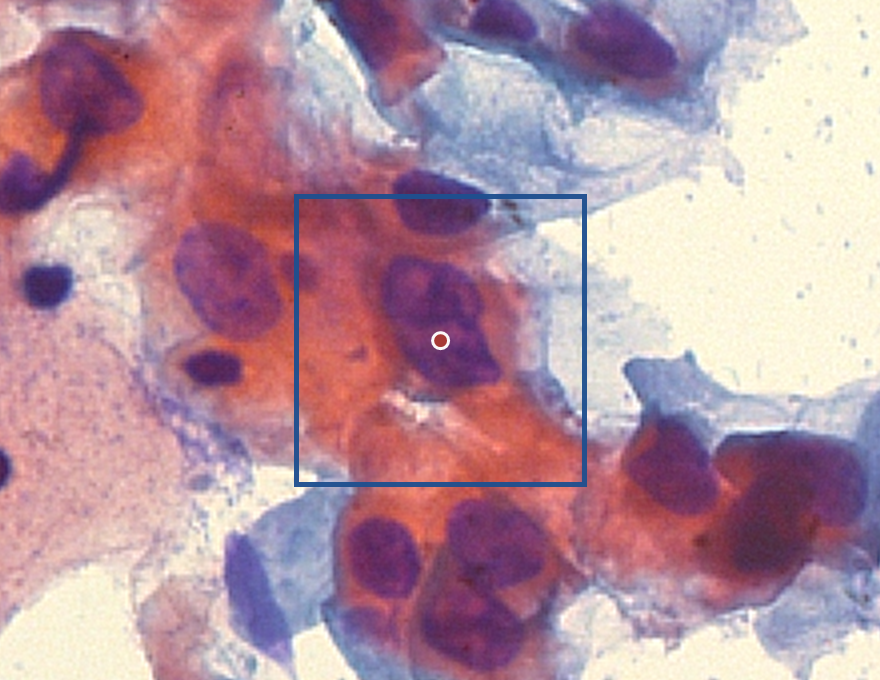
\includegraphics[width=.92\linewidth]{cric_point_box_zoom.png}
\vspace{.1cm}

{\scriptsize\color{muted}Ponto anotado no núcleo e região quadrada usada para treinar o detector.}

\column{.5\textwidth}
\vspace{.2cm}
{\Large\bfseries Hipótese testada}

\vspace{.25cm}
\begin{itemize}
  \item O centro vem da anotação.
  \item A extensão da região é definida no protocolo.
  \item Foram avaliados lados de 48 a 192 px.
\end{itemize}

\vspace{.35cm}
{\small\color{muted}A pergunta é como a forma de usar os pontos no treino afeta a localização e a contagem final.}
\end{columns}
\end{frame}

% 10
\tightframe{Partições e protocolo}
\begin{columns}[T,totalwidth=\textwidth]
\column{.52\textwidth}
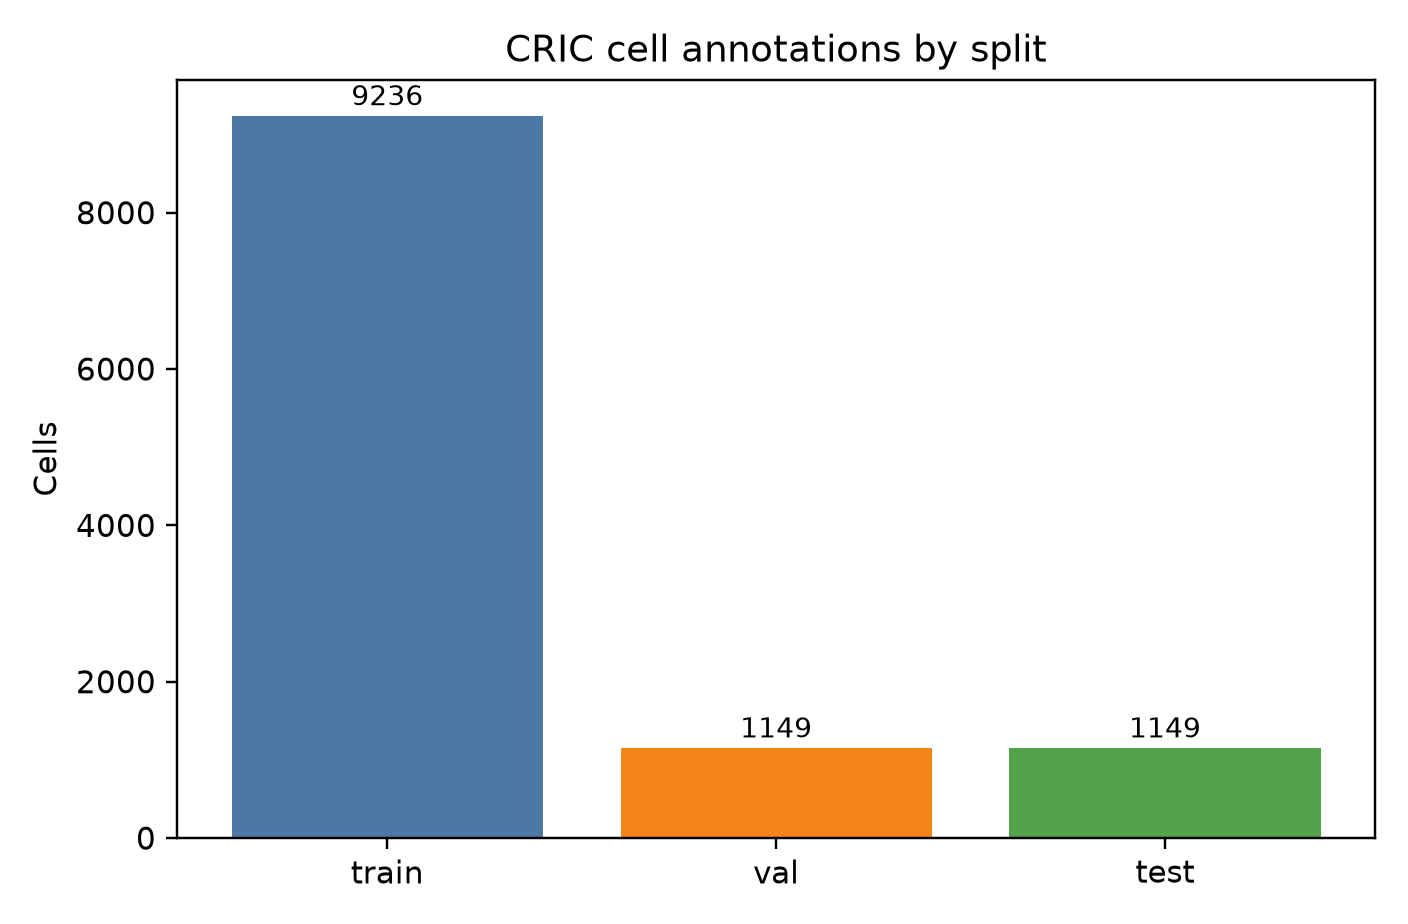
\includegraphics[width=.95\linewidth]{fig_particoes_celulas.png}

\column{.48\textwidth}
\metriccard{ufpiBlue}{Treino}{320}{9.236 células}
\hspace{.14cm}
\metriccard{ufpiGold}{Validação}{40}{1.149 células}

\vspace{.18cm}
\metriccard{fnRed}{Teste}{40}{1.149 células}

\vspace{.35cm}
\begin{itemize}
  \item Imagem é a unidade de separação.
  \item Nenhuma imagem é compartilhada entre partições.
  \item Bootstrap por imagem no teste.
\end{itemize}
\end{columns}
\end{frame}

% 11
\tightframe{Métricas}
\begin{columns}[T,totalwidth=\textwidth]
\column{.5\textwidth}
\centering
\begin{tikzpicture}[scale=.70,transform shape]
  \draw[ufpiGold,very thick,fill=white] (-1.25,-.85) rectangle (1.25,.85);
  \draw[tpGreen,very thick,fill=white,opacity=.82] (-.65,-.55) rectangle (1.85,1.15);
  \node[font=\bfseries,text=ufpiBlue] at (0,-1.25) {IoU};
  \node[text width=4.8cm,align=center,font=\small\color{muted}] at (0,-1.75)
    {sobreposição entre referência e predição};

  \begin{scope}[xshift=4.65cm]
    \fill[ufpiBlue!80] (0,0) circle (.08);
    \draw[fnRed,very thick] (0,0) circle (.85);
    \fill[tpGreen!80] (.48,.38) circle (.08);
    \draw[->,thick,tpGreen] (0,0) -- (.48,.38);
    \node[font=\bfseries,text=ufpiBlue] at (0,-1.25) {Distância};
    \node[text width=4.5cm,align=center,font=\small\color{muted}] at (0,-1.75)
      {centro predito perto do ponto nuclear};
  \end{scope}
\end{tikzpicture}

\column{.5\textwidth}
\vspace{.1cm}
\begin{itemize}
  \item Localização: AP50, F1, precisão, revocação.
  \item Contagem: MAE, RMSE, viés, correlação.
  \item Qualitativo: acertos, falsos positivos e omissões.
\end{itemize}

\vspace{.35cm}
{\bfseries Ideia:} localização e contagem se complementam; uma métrica isolada pode esconder erro operacional.
\end{columns}
\end{frame}

% 12
\tightframe{RQ1: uso dos pontos no treino}
\begin{columns}[T,totalwidth=\textwidth]
\column{.68\textwidth}
\begin{tikzpicture}
\begin{axis}[
  width=\linewidth,height=5.05cm,
  xlabel={Tamanho usado no treino (px)},
  ylabel={Desempenho},
  xmin=40,xmax=200,ymin=.62,ymax=.91,
  xtick={48,72,96,120,144,168,192},
  grid=major,grid style={black!8},
  legend style={draw=none,fill=white,font=\scriptsize,at={(.5,-.22)},anchor=north,legend columns=3},
  tick label style={font=\scriptsize},
  label style={font=\small}
]
\addplot[ufpiBlue,thick,mark=*] table[x=box_size_px,y=f1_val_iou50,col sep=comma]{../sbc-final/dados/bbox_sweep.csv};
\addlegendentry{F1@0,50}
\addplot[fpOrange,thick,dashed,mark=square*] table[x=box_size_px,y=ap50_val,col sep=comma]{../sbc-final/dados/bbox_sweep.csv};
\addlegendentry{AP50}
\addplot[tpGreen,thick,densely dotted,mark=triangle*] table[x=box_size_px,y=recall_val_iou50,col sep=comma]{../sbc-final/dados/bbox_sweep.csv};
\addlegendentry{Revocação}
\addplot[only marks,mark=*,mark size=3pt,ufpiGold] coordinates {(144,0.8228176)};
\end{axis}
\end{tikzpicture}

\column{.32\textwidth}
\vspace{.45cm}
{\Large\bfseries Platô, não ponto mágico}

\vspace{.3cm}
\begin{itemize}
  \item F1 estável entre 96 e 192 px.
  \item 160 px teve supercontagem.
  \item 144 px foi escolha operacional.
\end{itemize}
\end{columns}
\end{frame}

% 13
\tightframe{RQ2: escala YOLO11}
\centering
\begin{tikzpicture}[node distance=.5cm]
  \node[draw=ufpiBlue!45,fill=white,rounded corners=9pt,text width=3.35cm,minimum height=3.55cm,inner sep=8pt] (n) {
    {\Large\bfseries YOLO11n}\\[7pt]
    {\small F1: \bfseries 0,823}\\
    {\small AP50: \bfseries 0,877}\\
    {\small MAE: \bfseries 4,83}\\[5pt]
    {\scriptsize\color{muted}Próximo e leve}
  };
  \node[right=.55cm of n,draw=tpGreen!55,fill=white,rounded corners=9pt,text width=3.35cm,minimum height=3.95cm,inner sep=8pt] (s) {
    {\Large\bfseries YOLO11s}\\[7pt]
    {\small F1: \bfseries 0,836}\\
    {\small AP50: \bfseries 0,885}\\
    {\small MAE: \bfseries 4,68}\\[5pt]
    {\scriptsize\color{tpGreen!70!black}\bfseries Melhor equilíbrio}
  };
  \node[right=.55cm of s,draw=fpOrange!60,fill=white,rounded corners=9pt,text width=3.35cm,minimum height=3.55cm,inner sep=8pt] (m) {
    {\Large\bfseries YOLO11m}\\[7pt]
    {\small F1: \bfseries 0,794}\\
    {\small Rev.: \bfseries 0,892}\\
    {\small MAE: \bfseries 8,13}\\[5pt]
    {\scriptsize\color{muted}Mais FP e supercontagem}
  };
  \draw[very thick,tpGreen] ([xshift=-.12cm,yshift=-.12cm]s.south west) rectangle ([xshift=.12cm,yshift=.12cm]s.north east);
\end{tikzpicture}

\vspace{.35cm}
{\small\color{muted}A escolha é operacional neste experimento, não uma afirmação universal de superioridade arquitetural.}
\end{frame}

% 14
\tightframe{Limiar operacional}
\begin{columns}[T,totalwidth=\textwidth]
\column{.66\textwidth}
\begin{tikzpicture}
\begin{axis}[
  width=\linewidth,height=5.05cm,
  xlabel={Confiança},
  ylabel={Métrica na validação},
  xmin=.02,xmax=.52,ymin=.28,ymax=1,
  xtick={.03,.10,.20,.35,.50},
  grid=major,grid style={black!8},
  legend style={draw=none,fill=white,font=\scriptsize,at={(.5,1.03)},anchor=south,legend columns=3},
  tick label style={font=\scriptsize},
  label style={font=\small}
]
\addplot[ufpiBlue,thick,mark=*] table[x=conf,y=F1,col sep=comma]{dados/limiares_iou50.csv};
\addlegendentry{F1}
\addplot[fpOrange,thick,dashed,mark=square*] table[x=conf,y=Precisao,col sep=comma]{dados/limiares_iou50.csv};
\addlegendentry{Precisão}
\addplot[tpGreen,thick,densely dotted,mark=triangle*] table[x=conf,y=Revocacao,col sep=comma]{dados/limiares_iou50.csv};
\addlegendentry{Revocação}
\draw[ufpiGold,very thick] (axis cs:.35,.28) -- (axis cs:.35,1);
\end{axis}
\end{tikzpicture}

\column{.34\textwidth}
\vspace{.45cm}
\metriccard{ufpiGold}{Limiar escolhido}{0,35}{validação}

\vspace{.3cm}
\begin{itemize}
  \item Baixo: quase tudo aparece, mas sobram FP.
  \item Alto: precisão sobe, revocação cai.
  \item 0,35 maximiza F1@0,50.
\end{itemize}
\end{columns}
\end{frame}

% 15
\tightframe{RQ3: teste retido}
\centering
\metriccard{ufpiBlue}{AP50}{0,8723}{IC95\% [0,843; 0,904]}
\hspace{.22cm}
\metriccard{tpGreen}{F1}{0,8190}{IC95\% [0,796; 0,842]}
\hspace{.22cm}
\metriccard{fpOrange}{MAE}{4,68}{células/imagem}
\hspace{.22cm}
\metriccard{ufpiGold}{Correlação}{0,9434}{contagem}

\vspace{.7cm}
\begin{tikzpicture}
  \node[draw=ufpiBlue!45,fill=white,rounded corners=9pt,text width=10.6cm,align=center,inner sep=10pt] {
    \Large\bfseries YOLO11s + região 144 px + confiança 0,35\\[3pt]
    \normalsize\color{muted}Configuração escolhida na validação e aplicada ao teste sem novo ajuste.
  };
\end{tikzpicture}
\end{frame}

% 16
\tightframe{Leitura operacional no teste}
\begin{columns}[T,totalwidth=\textwidth]
\column{.43\textwidth}
{\Large\bfseries Totais do teste}

\vspace{.25cm}
\begin{tikzpicture}
  \node[draw=ufpiBlue!40,fill=white,rounded corners=8pt,text width=4.65cm,inner sep=8pt] {
    \bfseries Teste retido completo\\[-1pt]
    \normalfont 40 imagens\\
    1.149 células anotadas\\
    1.232 detecções do modelo
  };
\end{tikzpicture}

\vspace{.5cm}
\begin{tikzpicture}
  \node[draw=lineGray,fill=white,rounded corners=8pt,text width=4.65cm,inner sep=8pt] {
    \bfseries Como ler:\\[-1pt]
    \normalfont os valores da matriz são acumulados nas 40 imagens, e a média por imagem aparece abaixo.
  };
\end{tikzpicture}

\column{.57\textwidth}
{\Large\bfseries Matriz de auditoria}

\vspace{.25cm}
\renewcommand{\arraystretch}{1.35}
\begin{tabular}{>{\raggedright\arraybackslash}p{2.6cm}cc}
\toprule
 & \textbf{Predição} & \textbf{Sem predição}\\
\midrule
\textbf{Célula anotada} &
\cellcolor{tpGreen!12}\textbf{975 VP} &
\cellcolor{fnRed!10}\textbf{174 FN}\\
\textbf{Sem célula anotada} &
\cellcolor{fpOrange!12}\textbf{257 FP} &
--\\
\bottomrule
\end{tabular}

\vspace{.5cm}
\begin{tikzpicture}
  \node[draw=ufpiBlue!35,fill=white,rounded corners=8pt,text width=6.25cm,inner sep=8pt,align=center] {
    \bfseries Média por imagem:\\
    \normalfont 24,4 VP \hspace{.2cm} 6,4 FP \hspace{.2cm} 4,4 FN
  };
\end{tikzpicture}

\vspace{.2cm}
{\small\color{muted}Sem verdadeiro negativo: em detecção, o fundo não tem contagem finita.}
\end{columns}
\end{frame}

% 17
\tightframe{Exemplos qualitativos}
\centering
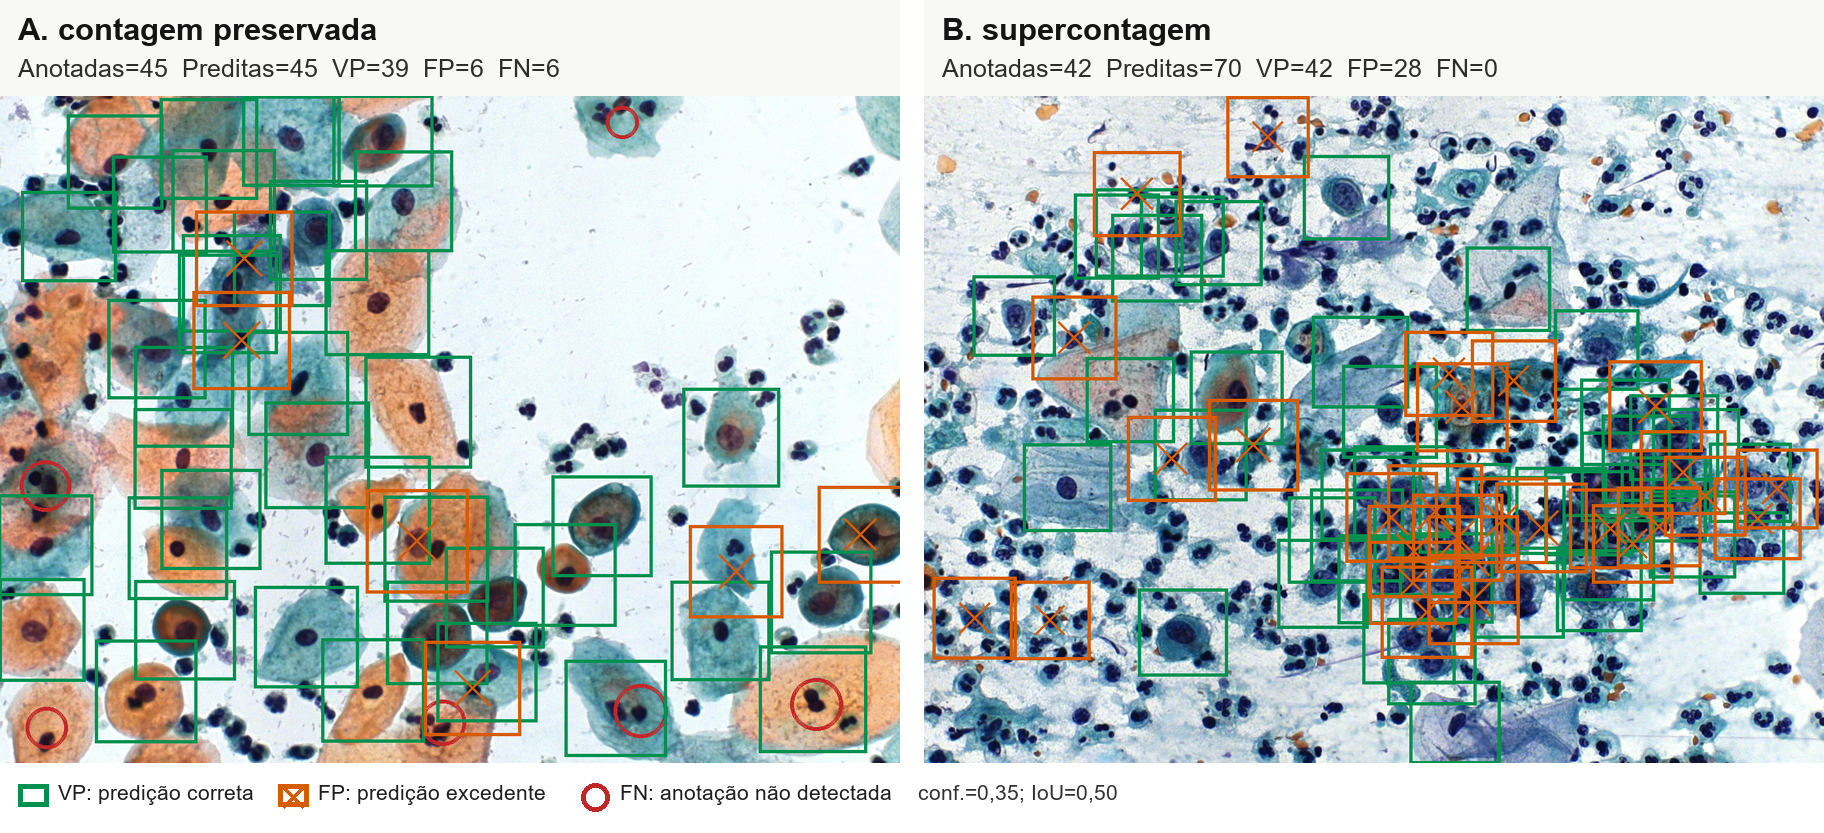
\includegraphics[width=.96\linewidth,height=6.05cm,keepaspectratio]{qualitativo_teste.png}

\vspace{.08cm}
\begin{tikzpicture}
  \node[draw=tpGreen,fill=white,rounded corners=5pt,inner sep=3pt] {\scriptsize VP: detecção correta};
  \node[xshift=3.35cm,draw=fpOrange,fill=white,rounded corners=5pt,inner sep=3pt] {\scriptsize FP: detecção excedente};
  \node[xshift=6.85cm,draw=fnRed,fill=white,rounded corners=5pt,inner sep=3pt] {\scriptsize FN: círculo vermelho};
\end{tikzpicture}
\end{frame}

% 18
\tightframe{Conclusão}
\begin{columns}[T,totalwidth=\textwidth]
\column{.58\textwidth}
{\Large\bfseries Conclusão científica}

\vspace{.14cm}
\begin{itemize}
  \item Anotações pontuais podem sustentar um detector de células cervicais quando o protocolo explicita como os pontos são usados.
  \item O melhor ponto operacional combinou YOLO11s, limiar 0,35 e avaliação no teste retido.
  \item Localização e contagem contam partes diferentes da história; por isso, precisam ser reportadas juntas.
\end{itemize}

\vspace{.08cm}
\begin{tikzpicture}
  \node[draw=ufpiBlue!45,fill=softBlue,rounded corners=6pt,text width=7.0cm,inner sep=5pt] {
    {\bfseries Ideia central}\\[3pt]
    {\small O foco não é a ``melhor caixa'', mas a construção de um caminho auditável para detectar e contar células a partir de uma base anotada por pontos.}
  };
\end{tikzpicture}

\column{.42\textwidth}
\centering
\metriccard{ufpiBlue}{AP50 no teste}{0,8723}{localização}
\hspace{.12cm}
\metriccard{tpGreen}{F1 no teste}{0,8190}{equilíbrio}

\vspace{.25cm}
\metriccard{fpOrange}{MAE}{4,68}{contagem}
\hspace{.12cm}
\metriccard{ufpiBlue}{Correlação}{0,9434}{contagem}

\vspace{.35cm}
\begin{tikzpicture}[
  font=\small
]
  \node[draw=lineGray,fill=white,rounded corners=6pt,text width=4.7cm,align=left,inner sep=8pt] {
    {\bfseries Limite assumido}\\[3pt]
    {\scriptsize O sistema não é diagnóstico: ele organiza evidências para localização, contagem e revisão assistida.}
  };
\end{tikzpicture}
\end{columns}
\end{frame}

% 19
\tightframe{Entregáveis e repositório}
\begin{columns}[T,totalwidth=\textwidth]
\column{.53\textwidth}
{\Large\bfseries Estrutura entregue}

\vspace{.12cm}
\begin{tikzpicture}[
  font=\scriptsize,
  folder/.style={draw=ufpiBlue!35,fill=softBlue,rounded corners=1pt,minimum width=.24cm,minimum height=.16cm,inner sep=0pt},
  file/.style={draw=muted!45,fill=white,rounded corners=.5pt,minimum width=.18cm,minimum height=.22cm,inner sep=0pt}
]
  \node[draw=lineGray,fill=white,rounded corners=6pt,minimum width=6.35cm,minimum height=4.5cm,anchor=north west] at (0,0) {};
  \node[anchor=west,font=\scriptsize\bfseries\ttfamily] at (.25,-.32) {Pesquisa-Jean/};

  \draw[lineGray] (.52,-.52) -- (.52,-3.95);
  \foreach \y/\name/\tag in {
    -.75/LaTeX/artigo + slides,
    -1.25/src/cervical\_cell\_detection/pipeline,
    -1.75/results/article\_materials/resultados,
    -2.25/configs/experimentos,
    -2.75/docs/documentação,
    -3.25/README.md/guia do projeto,
    -3.75/run.ps1 + setup.ps1/reprodução
  } {
    \draw[lineGray] (.52,\y) -- (.78,\y);
    \node[anchor=west,font=\scriptsize\ttfamily] at (.88,\y) {\name};
    \node[anchor=west,font=\scriptsize\color{muted}] at (3.95,\y) {\tag};
  }
  \node[folder] at (.77,-.75) {};
  \node[folder] at (.77,-1.25) {};
  \node[folder] at (.77,-1.75) {};
  \node[folder] at (.77,-2.25) {};
  \node[folder] at (.77,-2.75) {};
  \node[file] at (.77,-3.25) {};
  \node[file] at (.77,-3.75) {};
\end{tikzpicture}

\vspace{.14cm}
\begin{tikzpicture}
  \node[draw=ufpiBlue!45,fill=white,rounded corners=6pt,text width=6.35cm,inner sep=6pt] {
    {\bfseries Repositório público}\\[-1pt]
    {\scriptsize\href{https://github.com/JeanCarlos899/Pesquisa-Jean}{github.com/JeanCarlos899/Pesquisa-Jean}}
  };
\end{tikzpicture}

\column{.47\textwidth}
\centering
{\Large\bfseries Artigo final}

\vspace{.12cm}
\begin{tikzpicture}
  \node[draw=lineGray,line width=.45pt,fill=white,inner sep=1.3pt] at (1.12,.34)
    {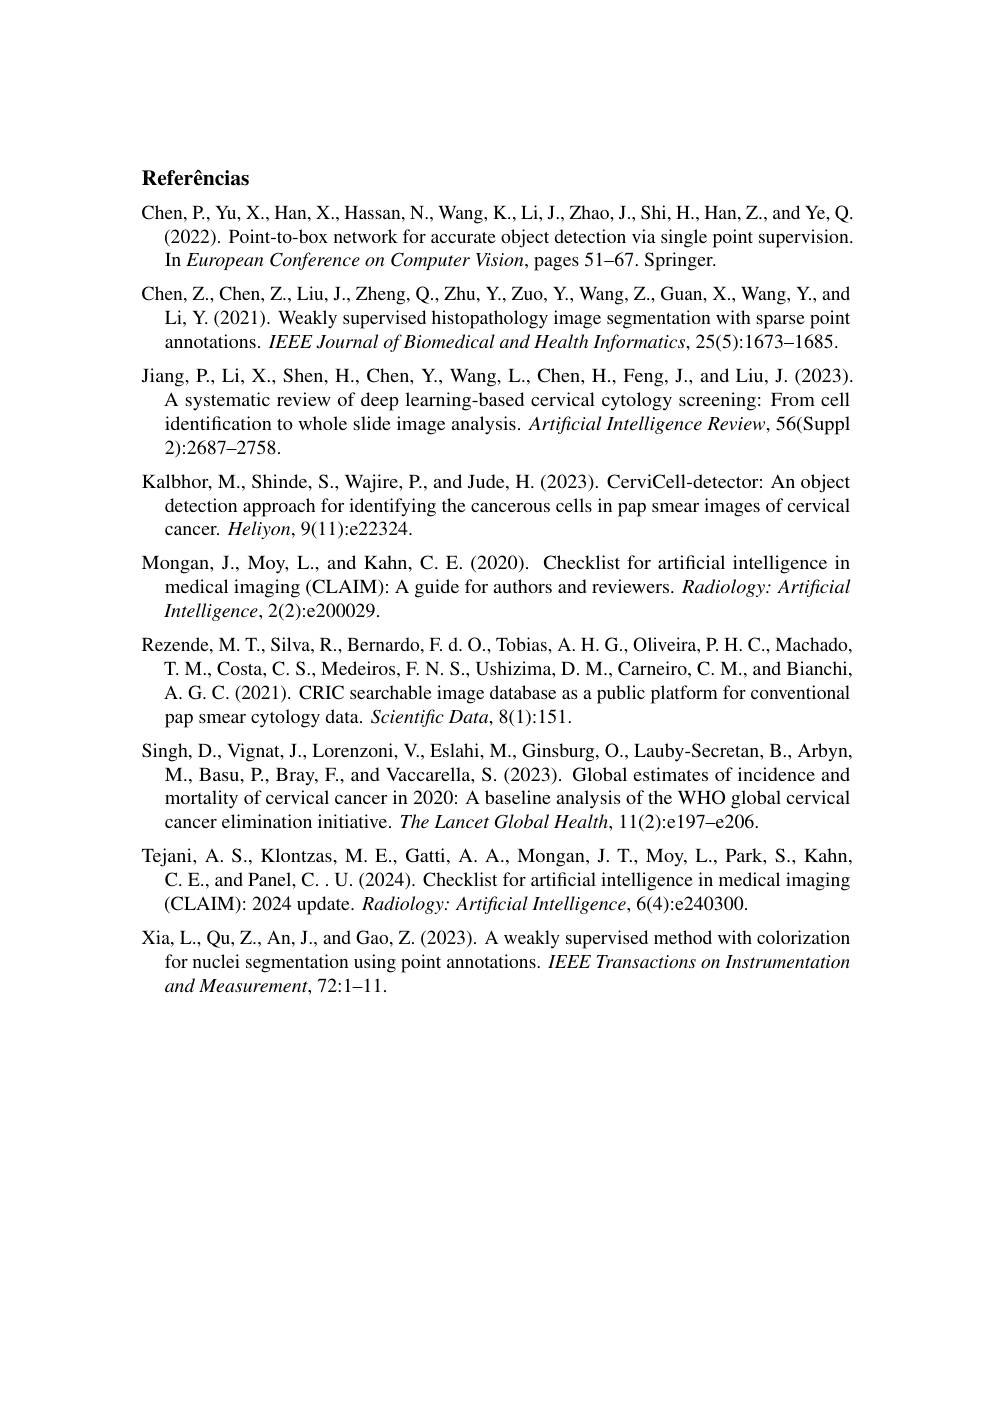
\includegraphics[height=4.05cm,trim=1.1cm 1.2cm 1.1cm 1.2cm,clip]{article_page-8.png}};
  \node[draw=lineGray,line width=.45pt,fill=white,inner sep=1.3pt] at (.08,-.04)
    {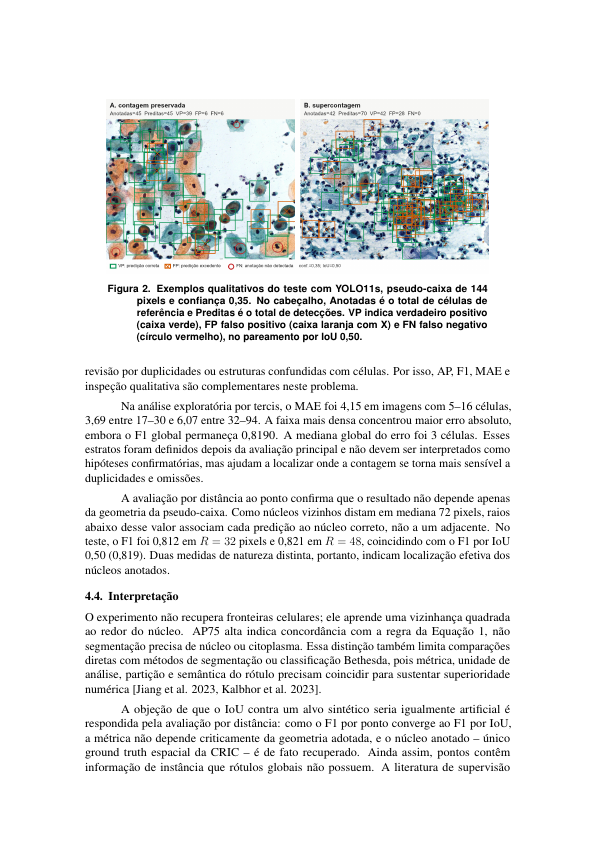
\includegraphics[height=4.08cm,trim=1.1cm 1.2cm 1.1cm 1.2cm,clip]{article_page-6.png}};
  \node[draw=ufpiBlue!45,line width=.85pt,fill=white,inner sep=2pt] at (-.96,-.43)
    {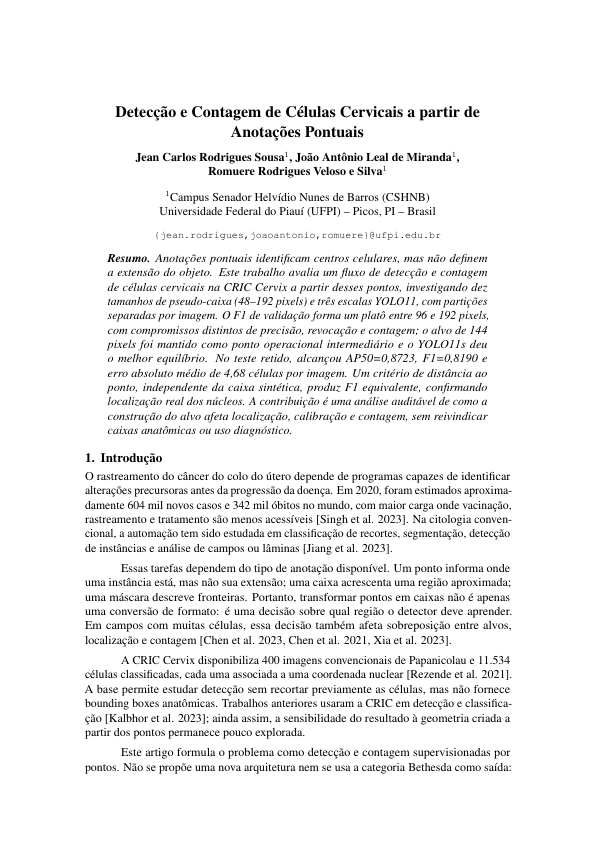
\includegraphics[height=4.08cm,trim=.8cm .9cm .8cm .9cm,clip]{article_page-1.png}};
  \node[fill=white,draw=ufpiBlue!30,rounded corners=5pt,text width=4.45cm,align=center,inner sep=4pt] at (.05,-3.08)
    {\scriptsize\color{muted}Template SBC, 8 páginas, resultados e referências.};
\end{tikzpicture}
\end{columns}
\end{frame}

\backuptrue
\appendix
\setcounter{framenumber}{1}

% Backup 1
\tightframe{Backup: hiperparâmetros}
\begin{columns}[T,totalwidth=\textwidth]
\column{.5\textwidth}
\begin{itemize}
  \item YOLO11n/s/m com pesos pré-treinados.
  \item AdamW, taxa inicial 0,002.
  \item Agendamento cossenoidal e precisão mista.
  \item Entrada nominal: 832 para n/s; 864 para m.
\end{itemize}

\column{.5\textwidth}
\begin{itemize}
  \item RQ1: até 35 épocas.
  \item RQ2: até 80 épocas, paciência 20.
  \item RTX 3060 Laptop, 6 GB VRAM.
  \item Artefatos persistidos por etapa.
\end{itemize}
\end{columns}
\end{frame}

% Backup 2
\tightframe{Backup: tabela completa do teste}
\centering
\begin{tabular}{lcc}
\toprule
Métrica & Valor & IC95\% \\
\midrule
Precisão & 0,7914 & [0,746; 0,833] \\
Revocação & 0,8486 & [0,822; 0,877] \\
F1 & 0,8190 & [0,796; 0,842] \\
AP30 & 0,8843 & [0,858; 0,913] \\
AP50 & 0,8723 & [0,843; 0,904] \\
AP75 & 0,7515 & [0,695; 0,811] \\
MAE & 4,675 & [3,150; 6,425] \\
RMSE & 7,216 & [4,560; 9,850] \\
Viés & 2,075 & [0,050; 4,126] \\
Correlação & 0,9434 & [0,874; 0,979] \\
\bottomrule
\end{tabular}
\end{frame}

% Backup 3
\tightframe{Backup: composição Bethesda}
\begin{columns}[T,totalwidth=\textwidth]
\column{.55\textwidth}
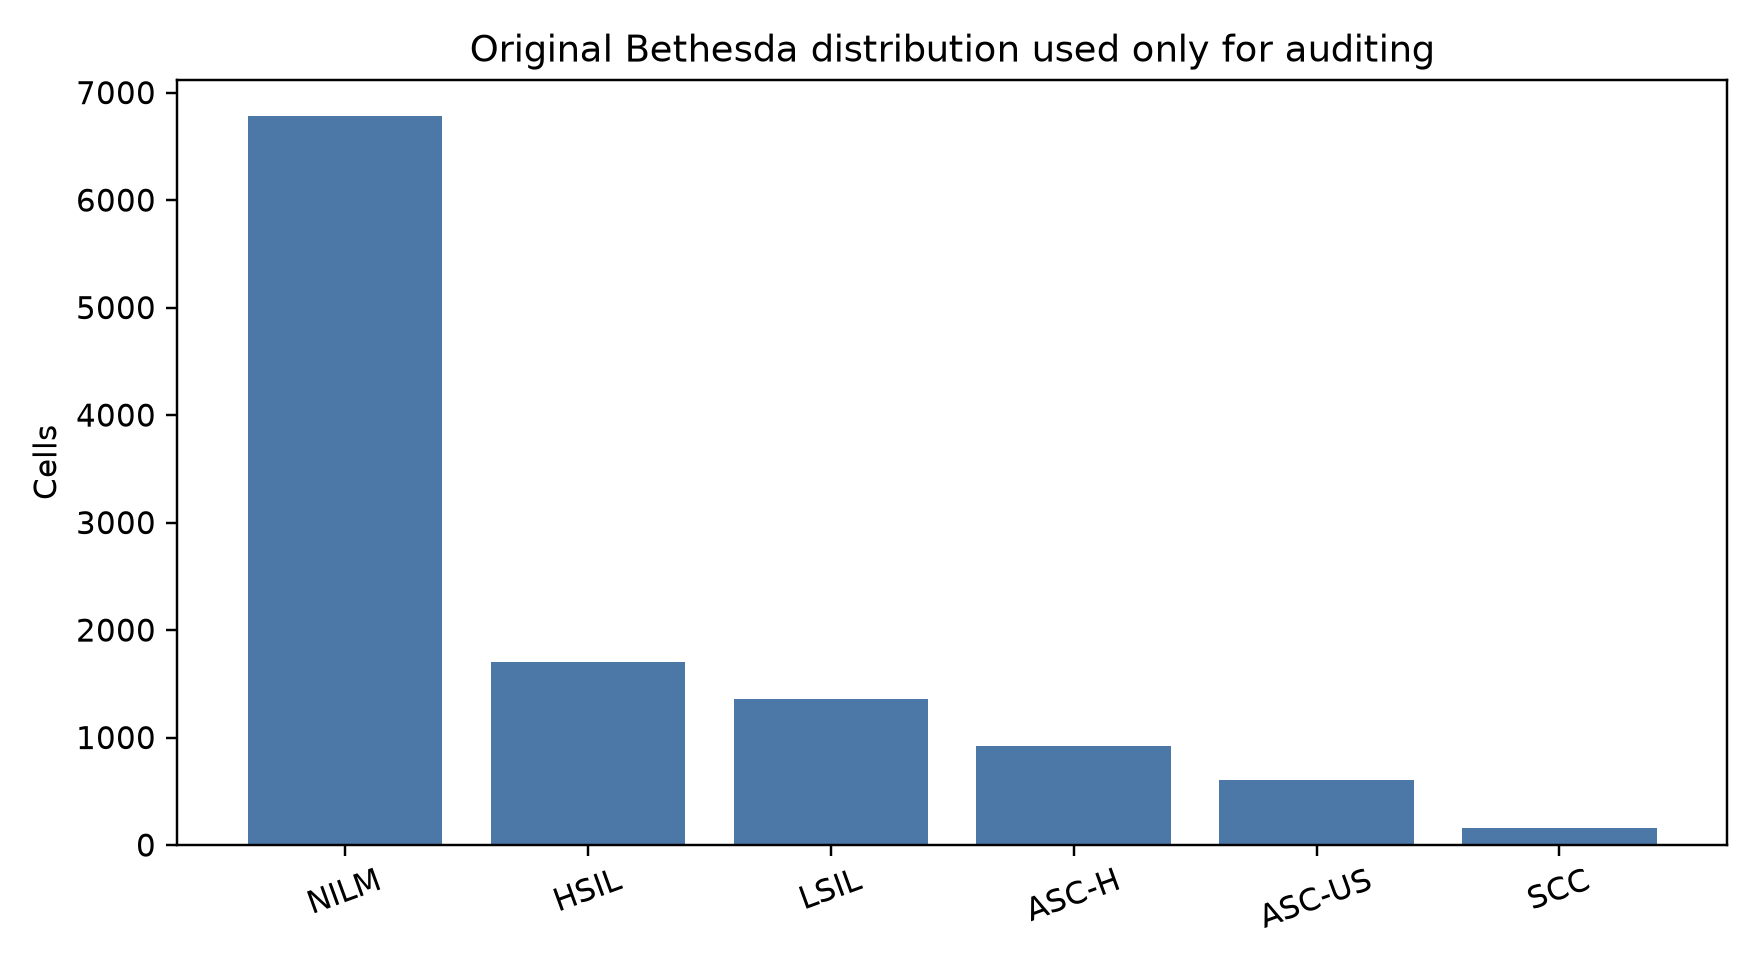
\includegraphics[width=.92\linewidth]{fig_composicao_bethesda_original.png}

\column{.45\textwidth}
\begin{itemize}
  \item A distribuição mostra heterogeneidade clínica.
  \item As classes não foram alvo do detector.
  \item O objetivo foi localizar qualquer célula anotada.
\end{itemize}
\end{columns}
\end{frame}

% Backup 4
\tightframe{Backup: por que classe única?}
\begin{tikzpicture}[>=Latex,scale=.84,transform shape]
  \node[draw=ufpiBlue!50,fill=white,rounded corners=8pt,text width=4cm,align=center,inner sep=8pt] (a)
    {Bethesda\\{\scriptsize\color{muted}informação clínica nos metadados}};
  \node[right=1.1cm of a,draw=ufpiGold!70,fill=white,rounded corners=8pt,text width=4cm,align=center,inner sep=8pt] (b)
    {Classe única\\{\scriptsize\color{muted}\textit{cell}}};
  \node[right=1.1cm of b,draw=tpGreen!55,fill=white,rounded corners=8pt,text width=4cm,align=center,inner sep=8pt] (c)
    {Localização\\{\scriptsize\color{muted}etapa antes de classificação}};
  \draw[->,thick,ufpiBlue] (a) -- (b);
  \draw[->,thick,ufpiBlue] (b) -- (c);
\end{tikzpicture}

\vspace{.45cm}
{\large\bfseries A pergunta do artigo é espacial, não diagnóstica.}
\end{frame}

% Backup 5
\tightframe{Backup: por que não segmentação?}
\begin{columns}[T,totalwidth=\textwidth]
\column{.5\textwidth}
{\Large\bfseries Ground truth disponível}
\vspace{.25cm}
\begin{itemize}
  \item Pontos nucleares.
  \item Sem regiões anatômicas delimitadas.
  \item Sem máscaras de núcleo/citoplasma.
\end{itemize}

\column{.5\textwidth}
{\Large\bfseries Interpretação correta}
\vspace{.25cm}
\begin{itemize}
  \item AP75 mede aderência à região de referência.
  \item F1 por distância confirma localização do ponto.
  \item Não há reivindicação diagnóstica.
\end{itemize}
\end{columns}
\end{frame}

% Backup 6
\tightframe{Backup: reprodutibilidade}
\begin{columns}[T,totalwidth=\textwidth]
\column{.55\textwidth}
\begin{itemize}
  \item Splits por imagem.
  \item Metadados das regiões de treino.
  \item CSVs e tabelas de métricas.
  \item Predições do teste.
  \item Materiais do artigo.
\end{itemize}

\column{.45\textwidth}
\begin{tikzpicture}
  \node[draw=ufpiBlue!50,fill=white,rounded corners=8pt,text width=5.1cm,inner sep=9pt] {
    {\bfseries GitHub}\\[3pt]
    \url{github.com/JeanCarlos899/Pesquisa-Jean}\\[6pt]
    {\scriptsize\color{muted}Repositório público do projeto.}
  };
\end{tikzpicture}
\end{columns}
\end{frame}

\end{document}
